\section{轴三维模型构建}\label{sec:zhoujianmo}

在\ref{sec:zhoufengxi}节中提出了叠加建模和运用包含关建模两种方式构建轴零件的三维模型。两种方试对于图\ref{fig:xiaolunzhou}所示的轴零件而言,其建模过程都很简单,其差别主要是选择的组合点不一样。本节主以叠加建模法介绍轴零件的建模过程,读者可若有兴趣可自行实践运用包含关系建模法。

\begin{procedure}
\item 将视图方向切换为左视图

尽管图\ref{fig:xiaolunzhou}所示的轴零件仅仅只有一个视图,但是根据构建模套筒三维模型的经验,可知表达其回转体特征的视图位于左视图,故需要先将视图方向切换为左视图,以保证零件三维模型的主视图与零件图的主视图方向一致。
\begin{lstlisting}
命令: -VIEW
输入选项 [?/删除(D)/正交(O)/恢复(R)/保存(S)/设置(E)/窗口(W)]: left
\end{lstlisting}

\item 将视图方向切换为西南等轴测

为了方便观察三维模型的构建,需要将再次将视图切换为西南等轴测,此时AutoCAD的坐标状态由平面直角坐标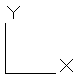
\includegraphics[scale=0.2]{twoaxis.png} 变为三维直角坐标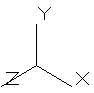
\includegraphics[scale=0.15]{threeaxis.png}。值得注意的是此时X轴和Y轴位于左视图的位置。

\begin{lstlisting}
命令: -VIEW
输入选项 [?/删除(D)/正交(O)/恢复(R)/保存(S)/设置(E)/窗口(W)]: swiso
\end{lstlisting}

\yaodian{仔细观察三维坐标系中X轴和Y轴的位置对于准确构建三维模型是十分必要的,可以避免许多不必要的错误。}
\item 构建$\phi 16$圆柱体

我们按照由大到小的顺序开始构建轴零件的各个部分,首先构建$\phi 16$圆柱体,其结果如图\ref{fig:zhoufirst}所示。
\begin{lstlisting}
命令: CYLINDER
指定底面的中心点或 [三点(3P)/两点(2P)/切点、切点、半径(T)/椭圆(E)]:
指定底面半径或 [直径(D)]: 8
指定高度或 [两点(2P)/轴端点(A)]: 2
\end{lstlisting}

\begin{figure}[htbp]
\centering
\subfloat[]{\label{fig:zhoufirst}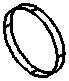
\includegraphics[scale=0.7]{zhoufirst.png}}\hspace{30pt}
\subfloat[]{\label{fig:zhoufirstselect}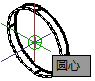
\includegraphics[scale=0.7]{zhoufirstselect.png}}\hspace{30pt}
\subfloat[]{\label{fig:zhousecond}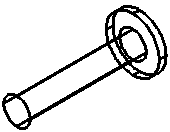
\includegraphics[scale=0.7]{zhousecond.png}}
\caption{轴三维模型构建过程一}
\end{figure}
\item 构建$\phi 8$圆柱体

接下来,按照图\ref{fig:zhoufirstselect}所示位置选择$\phi 16$圆柱体的圆心做为$\phi 8$圆柱体的底圆圆心,并以此构建$\phi 8$圆柱体,其结果如图\ref{fig:zhousecond}所示。

\begin{lstlisting}
命令: CYLINDER
指定底面的中心点或 [三点(3P)/两点(2P)/切点、切点、半径(T)/椭圆(E)]:

指定底面半径或 [直径(D)] <8.0000>: 4

指定高度或 [两点(2P)/轴端点(A)] <2.0000>: 35
\end{lstlisting}
\item 构建$\phi 6$圆柱体

接下来,按照图\ref{fig:zhousecondselect}所示位置选择$\phi 8$圆柱体的圆心做为$\phi 6$圆柱体的底圆圆心,并以此构建$\phi 6$圆柱体,其结果如图\ref{fig:zhouthree.}所示。

\begin{figure}[htbp]
\centering
\subfloat[]{\label{fig:zhousecondselect}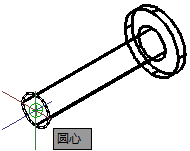
\includegraphics[scale=0.7]{zhousecondselect.png}}\hspace{30pt}
\subfloat[]{\label{fig:zhouthree.}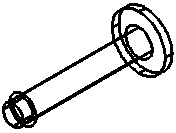
\includegraphics[scale=0.7]{zhouthree.png}}
\caption{轴三维模型构建过程二}
\end{figure}

\begin{lstlisting}
命令: CYLINDER
指定底面的中心点或 [三点(3P)/两点(2P)/切点、切点、半径(T)/椭圆(E)]:
指定底面半径或 [直径(D)] <4.0000>: 3
指定高度或 [两点(2P)/轴端点(A)] <35.0000>: 3
\end{lstlisting}
\item 合并实体

致此,我们已经分段构建了轴零件的三维模型,但是这些实体然是独立存在的,并没构成一个整体,因此需要将其合并为一个实体。在AutoCAD中,将多个实体合并的一个实体的命令是并集命令,其启动方法有:
\begin{itemize}
\item 键盘输入UNION\index{union,并集}或UNI。
\item 【修改】$\rightarrow$【实体编辑】$\rightarrow$【并集】
\item 【实体编辑】$\triangleright$【并集】图标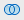
\includegraphics[scale=0.7]{union.png}。
\end{itemize}

启动命令后,按照图\ref{fig:unionselect}所示方式框选轴的3个组成部分,选择完后会以图\ref{fig:unionselectreult}所示的虚线形式表示被选中的对象。结束命令后,3个实体合并为一个整体,结果如图\ref{fig:unionresult}所示。
\begin{lstlisting}
命令:  UNION
选择对象: 指定对角点: 找到 3 个
选择对象:
\end{lstlisting}
\begin{figure}[htbp]
\centering
\subfloat[]{\label{fig:unionselect}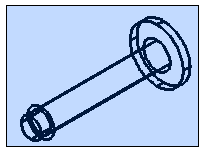
\includegraphics[scale=0.7]{unionselect.png}}\hspace{20pt}
\subfloat[]{\label{fig:unionselectreult}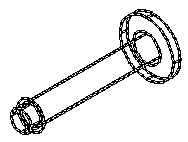
\includegraphics[scale=0.7]{unionselectreult.png}}\hspace{20pt}
\subfloat[]{\label{fig:unionresult}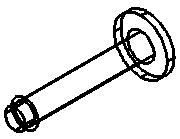
\includegraphics[scale=0.7]{unionresult.png}}
\caption{轴实体并集操作}
\end{figure}

\item 轴倒角

由于被倒角的两个位置,并不位于现一个平面之内,因此需要分两次进行,首先倒图\ref{fig:zhouchamferedge1}所示$\phi 6$圆柱体的角。
\begin{lstlisting}
命令: CHAMFEREDGE
距离 1 = 1.0000,距离 2 = 1.0000
选择一条边或 [环(L)/距离(D)]: d
指定距离 1 或 [表达式(E)] <1.0000>: 0.5
指定距离 2 或 [表达式(E)] <1.0000>: 0.5
选择一条边或 [环(L)/距离(D)]:
选择同一个面上的其他边或 [环(L)/距离(D)]:
按 Enter 键接受倒角或 [距离(D)]:
\end{lstlisting}

\begin{figure}[htbp]
\centering
\subfloat[]{\label{fig:zhouchamferedge1}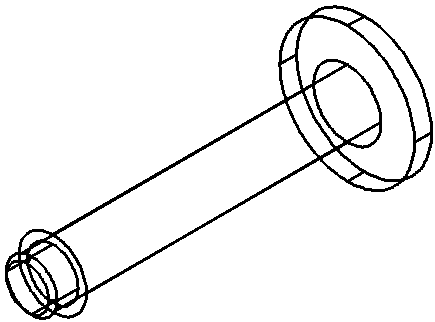
\includegraphics[scale=0.3]{zhouchamferedge1.png}}\hspace{20pt}
\subfloat[]{\label{fig:zhouchamferedge2}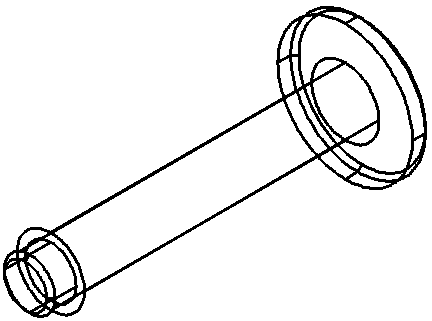
\includegraphics[scale=0.3]{zhouchamferedge2.png}}
\caption{轴倒角操作}
\end{figure}

接下来,倒$\phi 16$圆柱体的角,结果如图\ref{fig:zhouchamferedge2}所示。若要更清晰地看到$\phi 16$圆柱的倒角,可将视图方向切换为东南轴测进行观察。

\begin{lstlisting}
命令: CHAMFEREDGE
距离 1 = 0.5000,距离 2 = 0.5000
选择一条边或 [环(L)/距离(D)]:
选择同一个面上的其他边或 [环(L)/距离(D)]:
按 Enter 键接受倒角或 [距离(D)]:
\end{lstlisting}

\item 切换视觉样式为灰度

将视觉样式切换为灰度,其结果如图\ref{fig:zhouresult}所示。
\begin{lstlisting}
命令: VSCURRENT
输入选项 [二维线框(2)/线框(W)/隐藏(H)/真实(R)/概念(C)/着色(S)/带边缘着色(E)/灰度(G)/勾画(SK)/X 射线(X)/其他(O)] <二维线框>: g
\end{lstlisting}
\begin{figure}[htbp]
\centering
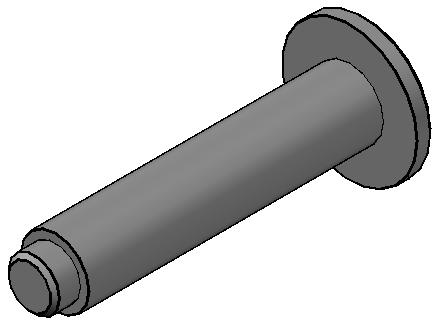
\includegraphics[scale=0.4]{zhouresult.png}
\caption{轴建模结果}\label{fig:zhouresult}
\end{figure}
\item 保存模型

将构建好的轴三维模型保存为“小轮组轴.dwg”。
\end{procedure}

\endinput